\begin{frame}[fragile]
	\frametitle{Multiple filenames}
			\begin{itemize}
				\item make long filenames short
				\item backward compatability
				\item file name aliases easy to read
			\end{itemize}
			\pause
			Usage examples

			\verb|find /etc -type l -exec ls -l {} \;|
			\begin{itemize}
				\item Hardlink
				\item Softlink (Symlink)
			\end{itemize}
\end{frame}

\begin{frame}[fragile]
	\frametitle{File links}
	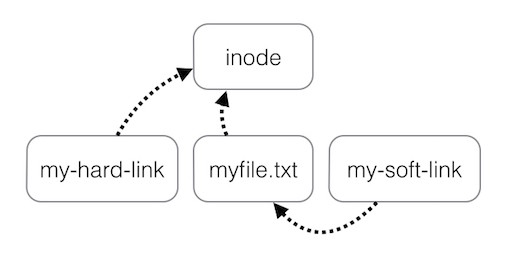
\includegraphics[height=0.4\textheight]{../../slides/cmdline/clipart/hardlink_softlink.jpg}
	\begin{block}{Hardlink}
	is a directory entry that associates a name with a file on a file system
        \end{block}
	\begin{block}{Softlink}
	any file that contains a reference to another file or directory 
	absolute or relative path 
        \end{block}
\end{frame}

\begin{frame}[fragile]
	\frametitle{How to create links}
	\begin{block}{Command ln}
		\begin{itemize}
			\item {\tt ln source target}
			\item {\tt ln -s source target}
		\end{itemize}
        \end{block}
	Create links

	\begin{lstlisting}
touch doc 
ln doc hardlink_file
ln -s doc softlink_file
ls -l
ls -li
stat doc hardlink_file softlink_file
\end{lstlisting}
\end{frame}

\begin{frame}[fragile]
	\frametitle{Hardlink limitation}
	\begin{lstlisting}
ls /boot/vmlinuz*
ln /boot/vmlinuz* ./kernel # <- error
ln -s /boot/vmlinuz* ./kernel
\end{lstlisting}
\end{frame}

\begin{frame}[fragile]
	\frametitle{Remove examples}
	Remove symlink target 

	{\tt rm doc} 

	{\tt ls -l}

	Remove hardlink

	\verb|stat hardlink_file|
\end{frame}
